\documentclass[conference]{IEEEtran}
\IEEEoverridecommandlockouts

\usepackage{cite}
\usepackage{amsmath,amssymb}
\usepackage{graphicx}
\usepackage{booktabs}
\usepackage{xcolor}
\usepackage{tikz}
\usetikzlibrary{arrows.meta,positioning,fit,backgrounds}
\usepackage[hidelinks]{hyperref}
\usepackage{url}

\definecolor{acc}{HTML}{C4501E}
\definecolor{boxfill}{HTML}{F6F5F2}
\definecolor{boxline}{HTML}{C9C6C0}

\begin{document}

\title{A Serially-Streamed KV-Cache Compression and\\
Eviction Coprocessor on GF180MCU,\\
Taken from RTL to GDS by an LLM Agent}

\author{\IEEEauthorblockN{Chaithu Talasila}
\IEEEauthorblockA{\textit{Longhorn Silicon (Team A71)} \\
\textit{The University of Texas at Austin}\\
Austin, TX, USA \\
talasila.chaithu1@gmail.com}}

\maketitle

\begin{abstract}
The key/value (KV) cache is the dominant memory- and bandwidth-consumer of
autoregressive large language model (LLM) decoding: it grows linearly with
context length and is re-read in its entirety at every generated token. We
present a compact coprocessor that moves three KV-cache maintenance operations
off the host and into dedicated silicon: (i) rotated INT3 \emph{value
compression} using a Walsh--Hadamard transform (WHT) and per-token scaling,
(ii) H2O heavy-hitter \emph{token-importance scoring} with single-victim
eviction, and (iii) a divide-free per-tile \emph{precision gate}. The block is
driven entirely over a four-wire SPI slave, keeping its pad footprint small
enough for a shared-reticle slot. We harden the design as a core-only
pre-integration macro on the GlobalFoundries 180\,nm (GF180MCU) open PDK using
the LibreLane flow. The implementation occupies $502.89\times520.81\,\mu\text{m}$
($0.262\,\text{mm}^2$, 7{,}080 standard cells) and passes signoff with zero
violations across Magic DRC, KLayout DRC, routing DRC, LVS, antenna, and layout
XOR. Distinctively, the entire RTL-to-GDS path---including diagnosing and
repairing a pin-naming audit failure, reordering pads for the assigned padframe
slot, and reconciling the delivered floorplan---was carried out by a large
language model (LLM) coding agent, with every step reproduced in continuous
integration. We report the architecture, the agentic design methodology, the
physical results, and an explicit account of what is and is not yet verified.
\end{abstract}

\begin{IEEEkeywords}
KV cache, LLM inference, hardware accelerator, quantization, Walsh--Hadamard
transform, GF180MCU, open-source EDA, LLM agents for chip design.
\end{IEEEkeywords}

\section{Introduction}
Autoregressive decoding in transformer-based LLMs caches the per-layer keys and
values of all previously seen tokens so that self-attention need not be
recomputed. This KV cache scales as $O(L\cdot d)$ in the number of cached tokens
$L$ and the per-token channel width $d$, and it is streamed in full for every
newly generated token. In deployment the KV cache, rather than the arithmetic,
becomes the binding constraint on memory footprint and off-chip bandwidth, and
the host expends a disproportionate share of its energy \emph{moving} the cache
rather than computing on it~\cite{h2o,kvquant}.

A large body of algorithmic work reduces this cost along two axes:
\emph{eviction}, which discards tokens predicted to be unimportant
(e.g.\ H2O's heavy-hitter oracle~\cite{h2o}), and \emph{quantization}, which
stores each cached value at low precision, often after a rotation that spreads
outliers across channels so that uniform quantizers behave
well~\cite{quarot,kvquant,kivi}. These techniques are almost always evaluated in
software. We instead ask what a small, dedicated silicon block that performs
this cache maintenance at the edge of memory looks like, and---because the
target is a Track~D (AI/LLM-for-circuits) shared-reticle tapeout---whether such a
block can be produced end-to-end by an LLM coding agent.

\noindent\textbf{Contributions.}
\begin{itemize}
\item A serially-streamed KV-cache coprocessor that unifies rotated INT3 value
compression, H2O token-importance/eviction, and a divide-free precision gate
behind a single four-wire SPI slave (Section~\ref{sec:arch}).
\item An agentic RTL-to-GDS methodology in which an LLM coding agent hardens the
design, diagnoses and repairs a physical pin-naming audit, reorders pads for the
assigned padframe slot, and reconciles the delivered floorplan---each step
reproduced in CI (Section~\ref{sec:method}).
\item A signoff-clean GF180MCU implementation ($0.262\,\text{mm}^2$, all checks
zero) with a calibrated statement of verification scope
(Sections~\ref{sec:results}--\ref{sec:limits}).
\end{itemize}

\section{Related Work}
\textbf{KV-cache eviction.} H2O~\cite{h2o} observes that a small set of
``heavy-hitter'' tokens accounts for most attention mass and can be identified by
accumulating per-token attention weights; low-mass tokens are evicted with little
quality loss. Our token-importance unit (TIU) implements this accumulate-then-argmin
policy directly in hardware.

\noindent\textbf{Rotated low-bit KV quantization.} QuaRot~\cite{quarot} and
related methods apply an orthogonal (Hadamard) rotation before quantization so
that per-channel outliers are redistributed, enabling aggressive uniform
quantization; KVQuant~\cite{kvquant} and KIVI~\cite{kivi} specialize such ideas to
the KV cache. Our value path (KVE) uses a Walsh--Hadamard transform followed by
per-token amax scaling and INT3 quantization, a synthesizable, division-light
realization of the same principle.

\noindent\textbf{LLM agents for chip design.} Language models have been applied to
RTL generation and EDA assistance~\cite{chipnemo}. We push further along the flow:
rather than generating a snippet, an agent drives an open-source
implementation flow~\cite{openlane} to a signoff-clean GDS and verifies its own
output against the physical database.

\section{Architecture}
\label{sec:arch}
Fig.~\ref{fig:arch} shows the block. A host streams work in over a standard
four-wire SPI slave (SCLK, CS\_n, MOSI, MISO); an on-chip loader exposes a
byte-addressed register fabric, and a compress-step finite-state machine (FSM)
sequences three hardened engines. Only ten functional signals plus power leave
the block, which is what allows it to fit a $1/8$ shared-reticle slot.

\begin{figure}[t]
\centering
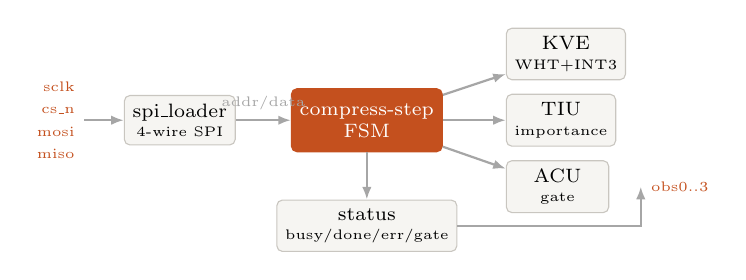
\begin{tikzpicture}[
  font=\scriptsize,
  box/.style={draw=boxline,fill=boxfill,rounded corners=2pt,align=center,
              minimum height=6mm,inner sep=3pt},
  hot/.style={draw=acc,fill=acc,text=white,rounded corners=2pt,align=center,
              minimum height=8mm,inner sep=3pt},
  w/.style={-{Latex[length=1.6mm]},gray!70,thick}]
  \node[box,minimum width=13mm] (spi) {spi\_loader\\[-1pt]\tiny 4-wire SPI};
  \node[hot,minimum width=15mm,right=7mm of spi] (fsm) {compress-step\\FSM};
  \node[box,minimum width=13mm,above right=1mm and 8mm of fsm] (kve) {KVE\\[-1pt]\tiny WHT+INT3};
  \node[box,minimum width=13mm,right=8mm of fsm] (tiu) {TIU\\[-1pt]\tiny importance};
  \node[box,minimum width=13mm,below right=1mm and 8mm of fsm] (acu) {ACU\\[-1pt]\tiny gate};
  \node[box,minimum width=15mm,below=6mm of fsm] (st) {status\\[-1pt]\tiny busy/done/err/gate};
  \node[left=5mm of spi,align=right,text=acc] (pins) {\tiny sclk\\\tiny cs\_n\\\tiny mosi\\\tiny miso};
  \draw[w] (pins) -- (spi);
  \draw[w] (spi) -- node[above]{\tiny addr/data} (fsm);
  \draw[w] (fsm) -- (kve);
  \draw[w] (fsm) -- (tiu);
  \draw[w] (fsm) -- (acu);
  \draw[w] (fsm) -- (st);
  \draw[w] (st.east) -| ([xshift=4mm]acu.east) node[right,text=acc]{\tiny obs0..3};
\end{tikzpicture}
\caption{Coprocessor block diagram. A four-wire SPI loader feeds a byte-addressed
fabric; the compress-step FSM (highlighted) orchestrates the KVE, TIU, and ACU
engines and exposes a four-bit status word on the observation pins.}
\label{fig:arch}
\end{figure}

\subsection{KVE: rotated INT3 value compression}
For each cached value token $\mathbf{v}\in\mathbb{R}^{d}$ (with $d$ a power of
two), the KVE applies a forward Walsh--Hadamard transform
$\mathbf{r}=\mathbf{H}_d\,\mathbf{v}$, computes a per-token maximum absolute value
$s=\max_i |r_i|$, and quantizes to a signed 3-bit code
\begin{equation}
c_i=\mathrm{clip}\!\left(\left\lfloor \frac{r_i}{s}\,(2^{b-1}-1)\right\rceil,\,-4,\,3\right),\quad b=3,
\end{equation}
emitting the $d$ INT3 codes together with a single \texttt{fp16} scale $s$; a
rotated \texttt{fp16} reconstruction $\hat{\mathbf{v}}$ is produced for read-back.
The transform spreads outliers across channels so the uniform INT3 grid is used
efficiently, echoing rotated-quantization results in
software~\cite{quarot,kvquant}. The datapath is fully synthesizable and
bit-exact against a behavioral reference; the combinational transform path is the
timing-critical path and sets the operating period.

\subsection{TIU: H2O token importance and eviction}
The TIU maintains a per-slot importance score by accumulating host-supplied
attention masses. On request it (i) emits a \emph{keep-tier} bitmap by
thresholding each slot's score and (ii) selects a single eviction victim as the
minimum-mass slot via a serialized argmin. This is a direct hardware realization
of the H2O heavy-hitter policy~\cite{h2o}.

\subsection{ACU: divide-free precision gate}
The ACU decides, per tile, whether the reconstructed values are ``peaky'' enough
to warrant retaining full \texttt{fp16} precision. It compares a scaled maximum
against the tile sum using only shifts, adds, and comparisons---no division---and
raises a single \texttt{gate\_fp16} bit.

\subsection{Serial interface and register map}
The loader implements SPI mode~0 (CPHA=0), MSB-first: a command byte
(WRITE/READ/START/STATUS) is followed by a 16-bit address and payload. The host
writes value tokens and attention masses, pulses START, polls STATUS, and reads
back the compressed records and decision byte (Table~\ref{tab:regmap}). Because
no output-only digital pad exists in the GF180 IO library, MISO and the four
observation bits are declared bidirectional and used as outputs.

\begin{table}[t]
\caption{Byte-addressed register map (fp16 little-endian).}
\label{tab:regmap}
\centering
\begin{tabular}{@{}lll@{}}
\toprule
Address & Region & Dir. \\
\midrule
\texttt{0x0300} & W --- per-token attention mass & write \\
\texttt{0x0400} & V --- value tokens (\texttt{fp16}) & write \\
\texttt{0x0800} & CODES --- rotated INT3 codes & read \\
\texttt{0x0A00} & SCALE --- per-token \texttt{fp16} scale & read \\
\texttt{0x0C00} & $\hat{\text{V}}$ --- rotated reconstruction & read \\
\texttt{0x0002} & DECISION --- \{gate, evict slot, keep\} & read \\
\texttt{0x0001} & STATUS mirror & read \\
\bottomrule
\end{tabular}
\end{table}

One \emph{compress step} therefore proceeds as: stream $L$ value tokens and
masses in; the KVE compresses every token to codes, scale, and reconstruction;
the TIU scores importance and selects a victim; the ACU sets the precision bit;
the host polls STATUS and reads the records back---all over the same four wires.

\section{Design Methodology: Agentic RTL-to-GDS}
\label{sec:method}
The distinguishing feature of this work (and its Track~D thesis) is that the
implementation flow was executed by an LLM coding agent rather than by hand. The
agent operated on the repository directly: reading the design and flow
configuration, editing HDL and YAML, running the physical-design flow inside a
container against the GF180MCU PDK, and---crucially---\emph{verifying its own
output against the physical database} rather than asserting success.

Two episodes are illustrative. First, a shared-reticle pin audit compares the
integrator's expected pin names character-for-character against the text labels
in the submitted GDS. An initial audit failed on six names because the status
port had been elaborated as a bus (\texttt{obs\_out[3:0]}, labelled
\texttt{obs\_out[0]}\ldots) while the pin list declared scalars
(\texttt{obs0}\ldots\texttt{obs3}), and because power had hardened as
\texttt{VDD}/\texttt{VSS} while the list declared \texttt{vdd}/\texttt{vss}. The
agent localized the root cause to naming (not logic), split the bus into four
scalar ports preserving bit order, aligned the power nets, re-hardened, and then
re-scanned the resulting GDS to confirm the labels
\texttt{obs0}\ldots\texttt{obs3} and \texttt{VDD}/\texttt{VSS} were present and no
\texttt{obs\_out[*]} remained. Second, on receiving the padframe floorplan for a
$1/8$ ``BV'' slot---which requires the chip-wide common ground on pin~1---the
agent reordered the pin list so that ground leads, and reconciled the delivered
floorplan against the pin list (both offered orientations matched exactly).

Every such step is reproduced by continuous integration, which reruns the
self-checking functional test and the full hardening on each push. The agent's
work is thus auditable rather than asserted: a third party can re-execute the
flow and obtain the same signoff.

\section{Implementation Results}
\label{sec:results}
The design is hardened as a core-only pre-integration macro (no padring or seal
ring) with the LibreLane Classic flow~\cite{openlane} on the open GF180MCU
PDK~\cite{gf180}, using the $5$\,V \texttt{gf180mcu\_fd\_sc\_mcu7t5v0} standard
cells. Fig.~\ref{fig:layout} shows the routed layout; Table~\ref{tab:results}
summarizes the physical metrics and signoff. All six signoff checks report zero
violations, and static timing closes with no setup or hold violations at the
target period.

\begin{figure}[t]
\centering
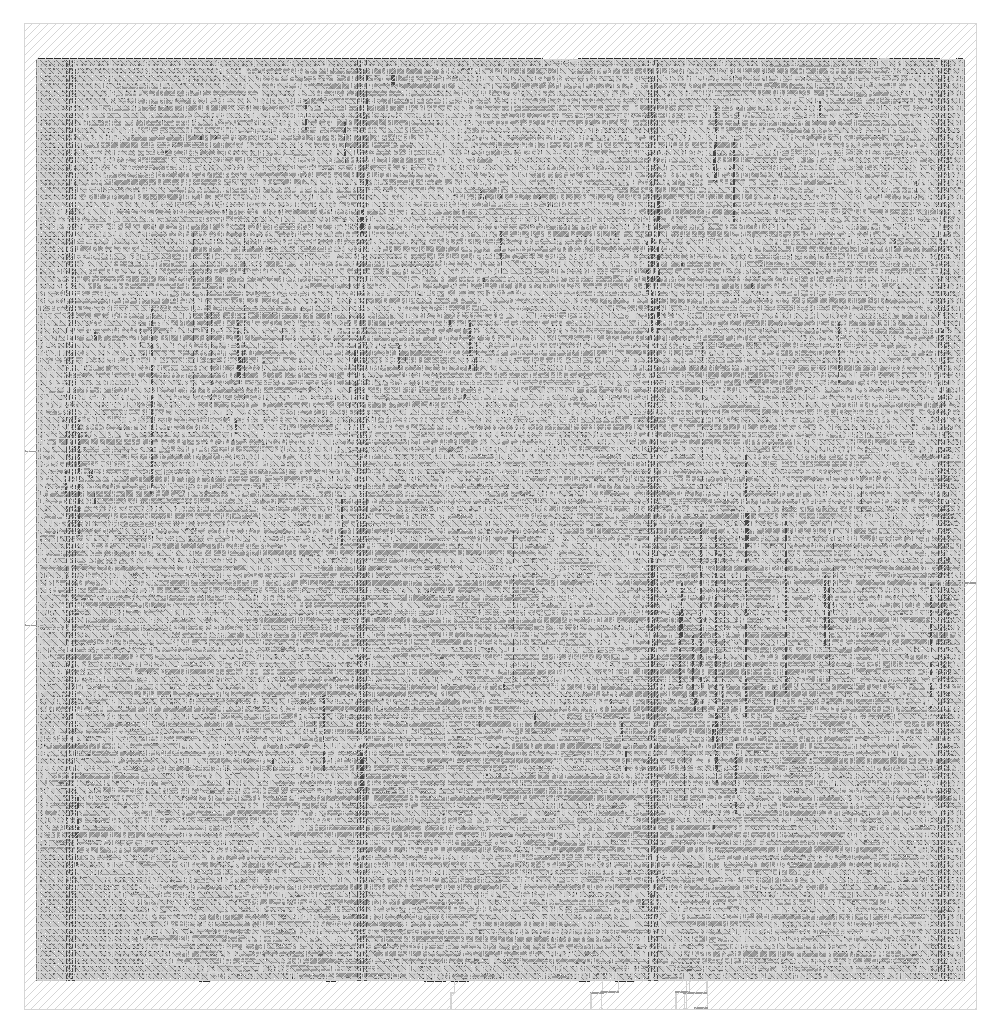
\includegraphics[width=0.72\columnwidth]{layout.png}
\caption{Routed GF180MCU layout of the core-only coprocessor
(\texttt{lambda\_kv\_coproc}), $502.89\times520.81\,\mu$m.}
\label{fig:layout}
\end{figure}

\begin{table}[t]
\caption{GF180MCU implementation and signoff.}
\label{tab:results}
\centering
\begin{tabular}{@{}ll@{}}
\toprule
Parameter & Value \\
\midrule
PDK / cells & gf180mcuD, 180\,nm / \texttt{mcu7t5v0} (5\,V) \\
Die area & $502.89\times520.81\,\mu\text{m}$ ($0.262\,\text{mm}^2$) \\
Standard cells & 7{,}080 ($\sim$62\% utilization) \\
Clock period & 300\,ns (setup/hold clean) \\
Magic DRC / KLayout DRC & 0 / 0 \\
Routing DRC / antenna & 0 / 0 \\
LVS / layout XOR & 0 / 0 \\
\bottomrule
\end{tabular}
\end{table}

The 300\,ns period ($\sim$3.3\,MHz) is set by the combinational Walsh--Hadamard
value path on this low-cost 180\,nm node; it is a deliberate area-for-speed
trade for a streaming maintenance block that is not on the model's arithmetic
critical path.

\section{Verification}
\label{sec:verif}
Functional correctness is established by a self-checking testbench that exercises
the complete SPI contract at the workshop tile size ($d{=}2$, $L{=}2$): it writes
importance masses and value tokens, issues START, polls STATUS to completion,
and reads back the decision byte, keep bitmap, and KVE codes/scale. The checks
are deterministic---FSM completion with the error flag clear, eviction victim
equal to the argmin of the masses, the keep bitmap equal to the per-slot
threshold test, INT3 codes within $[-4,3]$, and stable scale read-back---and all
pass. Layout-versus-schematic (LVS) ties the extracted layout back to the
synthesized netlist, so the GDS is a faithful realization of the verified RTL.
Both the functional test and the hardening are re-executed in CI on every push.

\section{Shared-Reticle Integration}
\label{sec:integ}
For the shared-reticle flow the team submits a core-only block plus a pin list;
the organizers generate the padframe, sized to the core area, and return a
floorplan (DEF) that the core is hardened into. Our twelve pins map onto a
$1/8$, 16-pin ``BV'' slot (Table~\ref{tab:pins}); the four unused slots are
auto-populated with analog pads by the integrator. The final GDS is pulled from
the project's default branch, combined with the other projects, and forwarded to
the channel partner---so integration is fully scripted and requires no manual
editing of the submitted layout.

\begin{table}[t]
\caption{BV-slot pin assignment (12 of 16 pins used).}
\label{tab:pins}
\centering
\begin{tabular}{@{}cll@{}}
\toprule
Pin & Signal & Pad / type \\
\midrule
1 & \texttt{VSS} & W12 / ground \\
2 & \texttt{clk} & W13 / Schmitt in \\
3--6 & \texttt{rst\_n}, \texttt{spi\_sclk/cs\_n/mosi} & W14--17 / in \\
7 & \texttt{spi\_miso} & W18 / bidir \\
8--11 & \texttt{obs0}--\texttt{obs3} & W19--22 / bidir \\
12 & \texttt{VDD} & N01 / power \\
\bottomrule
\end{tabular}
\end{table}

\section{Limitations and Future Work}
\label{sec:limits}
We state verification scope precisely. Correctness is established at the
\emph{RTL plus physical-signoff} level: RTL simulation of the SPI contract
together with LVS. We have \emph{not} run gate-level simulation of the
post-layout netlist, and the SPI testbench is a targeted deterministic
self-check rather than exhaustive coverage; bit-exactness of the KVE against its
behavioral reference is covered by block-level testbenches maintained separately.
Pad-level behavior (the core driving the physical pads through their
output-enable and configuration terminals) is handled by the integrator's
scripted padframe wiring and is not self-verified here. Finally, the design is
pre-fabrication: no silicon measurements exist. Natural next steps are
gate-level and post-layout timing simulation, a wider randomized functional
suite, and---after fabrication---bring-up over the same SPI link.

\section{Conclusion}
We presented a compact, serially-streamed KV-cache coprocessor that performs
rotated INT3 value compression, H2O token-importance/eviction, and a divide-free
precision gate behind a four-wire SPI slave, and hardened it to a signoff-clean
$0.262\,\text{mm}^2$ macro on the open GF180MCU node. The design was carried from
RTL to GDS by an LLM coding agent that repaired a physical pin-naming audit,
adapted to the assigned padframe slot, and verified its own output against the
GDS---with every step reproduced in continuous integration. The result argues
that agent-driven, open-source silicon implementation can produce auditable,
tapeout-ready blocks for shared-reticle programs.

\section*{Reproducibility}
The RTL, flow configuration, hardened GDS, and this paper are open at
\url{https://github.com/LonghornSilicon/gf180-longhorn-tiu}. Functional test:
\texttt{make sim-coproc}; hardening: \texttt{make coproc}.

\begin{thebibliography}{00}
\bibitem{h2o} Z. Zhang \textit{et al.}, ``H2O: Heavy-Hitter Oracle for Efficient
Generative Inference of Large Language Models,'' in \textit{Adv. Neural Inf.
Process. Syst. (NeurIPS)}, 2023.
\bibitem{quarot} S. Ashkboos \textit{et al.}, ``QuaRot: Outlier-Free 4-Bit
Inference in Rotated LLMs,'' in \textit{Adv. Neural Inf. Process. Syst.
(NeurIPS)}, 2024.
\bibitem{kvquant} C. Hooper \textit{et al.}, ``KVQuant: Towards 10 Million
Context Length LLM Inference with KV Cache Quantization,'' in \textit{Adv. Neural
Inf. Process. Syst. (NeurIPS)}, 2024.
\bibitem{kivi} Z. Liu \textit{et al.}, ``KIVI: A Tuning-Free Asymmetric 2bit
Quantization for KV Cache,'' in \textit{Proc. Int. Conf. Mach. Learn. (ICML)},
2024.
\bibitem{chipnemo} M. Liu \textit{et al.}, ``ChipNeMo: Domain-Adapted LLMs for
Chip Design,'' arXiv:2311.00176, 2023.
\bibitem{openlane} M. Shalan and T. Edwards, ``Building OpenLANE: A 130nm
OpenROAD-based Tapeout-Proven Flow,'' in \textit{Proc. IEEE/ACM Int. Conf.
Computer-Aided Design (ICCAD)}, 2020.
\bibitem{gf180} GlobalFoundries and Google, ``GF180MCU Open Source PDK,''
\url{https://github.com/google/gf180mcu-pdk}, 2022.
\end{thebibliography}

\end{document}
